% 1) Title
% 2) Date
% 3) Location
% 4) Present
% 5) Picture
% 6) Start Time
% 7) Stop Time
\insertmeeting 
	{Multimedia Maze} 
	{09/01/21}
	{Hagerty High School}
	{Annika, Falon, Samantha}
	{Images/RobotPics/robot.jpg}
	{3:30}
      {4:30}
	
\section*{Multimedia}
\noindent\hfil\rule{\textwidth}{.4pt}\hfil
\subsection*{Goals}
\begin{itemize}
    \item Future plans for communications such as social media posts, coming up with outreach ideas that we can work on

\end{itemize} 

\noindent\hfil\rule{\textwidth}{.4pt}\hfil

\subsection*{Accomplishments}
After the program meeting we worked on planing for new social media posts and future ideas on outreach. Ms. Po helped us and discussed with us the school’s goal for inclusion at Hagerty. Her words inspired us to come up with some other ideas for outreach and how we could show inclusion within our team and in our community. Multimedia is currently working on Team member takeover posts that will show what each member on the team is all about and how they contribute to the making of 4717. We brainstormed some of the things that we had to get done for a while such as sponsor letters. We also wrote some stuff that we had for outreach and ideas for communication that could bring robotics and STEM closer to the community. Not only that, but it would be cool to show that our team likes to have fun, so we even spent some time to come up with some team bonding activities we could do in the future. All in all, we simply brainstormed plans that we could make for the team throughout the season and posts for our social media. 
 

\begin{figure}[ht]
\centering
\begin{minipage}[b]{.50\textwidth}
  \centering
  
\includegraphics[width=0.8\textwidth]{Meetings/September/09-01-21/1.jpeg}
  \caption{New Account in Github}
  \label{fig:pic1}
\end{minipage}%
\hfill%
\begin{minipage}[b]{.50\textwidth}
  \centering
  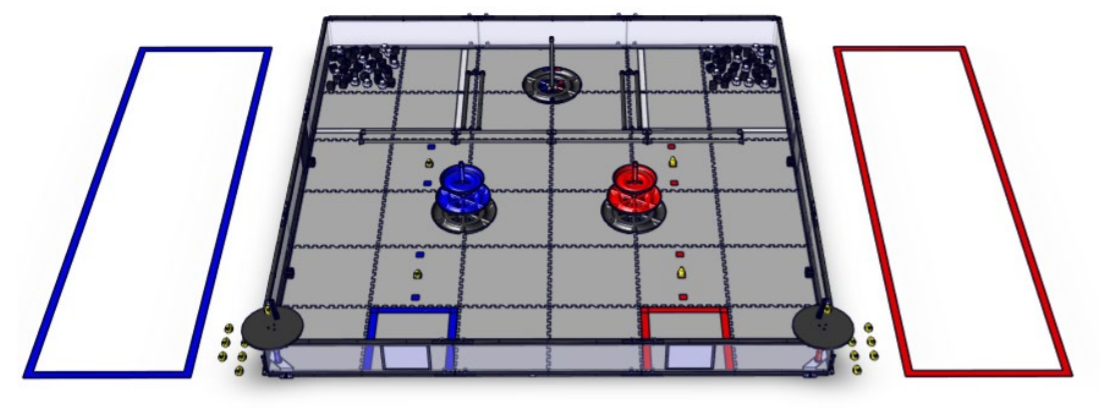
\includegraphics[width=0.8\textwidth]{Meetings/September/09-18-21/field.png}
  \caption{Screenshot of GitHub Repository}
  \label{fig:pic2}
\end{minipage}
\end{figure}












